\chapter{Nhận dạng tiếng nói}

\diary{19/01/2018: Hôm nay thực sự quá mệt với bạn Kaldi. Mãi không thể decode với các thuộc tính LDA-MLLT được? Hỏi mãi ở kaldi-help mà không có reply}

\diary{05/01/2018 - "điên đầu" với Sphinx và HTK. HTK thì đã bỏ rồi vì quá lằng nhằng. Sphinx thì setup được đối với dữ liệu nhỏ rồi. Nhưng không thể làm nó hoạt động với dữ liệu của VIVOS. Chắc hôm nay sẽ switch sang Kaldi vậy.}

\diary{26/12/2017 - Automatic Speech Recognition 100. Sau mấy ngày "vật lộn" với code base của Truong Do, thì cuối cùng cũng produce voice được. Cảm giác rất thú vị. Quyết định làm luôn ASR. Tìm mãi chẳng thấy code base đâu (chắc do lĩnh vực mới nên không có kinh nghiệm). May quá lại có bạn frankydotid có project về nhận diện tiếng Indonesia ở \href{https://github.com/frankydotid/Indonesian-Speech-Recognition}{github}. Trong README.md bạn đấy bảo là phải cần đọc HTK Book. Tốt quá đang cần cơ bản.}

Trong hệ thống nhận dạng tiếng nói, tín hiệu âm thanh được thu thập như những mẫu phù hợp cho quá trình xử lý của máy tính và được đưa vào quá trình nhận diện. Đầu ra của hệ thống là một câu phụ đề của câu nói.

Nhận dạng tiếng nói là một nhiệm vụ phức tạp và hệ thống tốt nhất trong nhận dạng tiếng nói rất phức tạp. Có rất nhiều cách tiếp cận cho mỗi thành phần. Trong phần này, người viết chỉ muốn đưa ra một cái nhìn tổng thể về nhận dạng tiếng nói, các khó khăn chính, các thành phần cơ bản, chức năng và tương tác của chúng trong một hệ thống nhận dạng tiếng nói.

\section{Các thành phần của hệ thống nhận dạng tiếng nói}

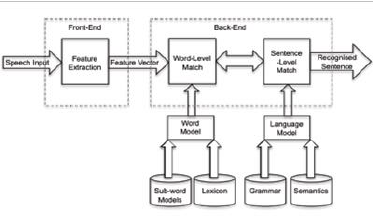
\includegraphics[width=10cm]{data_science/speech_recognition/asr_components}

Trong bước thứ nhất, trích rút thông tin \textit{Feature Extraction}, các mẫu tín hiệu được tham số hóa. Mục tiêu là trích xuất ra một tập các tham số (đặc trưng) từ tín hiệu có nhiều thông tin hữu ích nhất cho quá trình phân loại.  Các đặc trưng chính được trích xuất với điều kiện \textit{thích nghi} với các sự thay đổi của âm thanh và \textit{nhạy cảm} với các nội dung ngôn ngữ.

\definition{mô hình âm học}{Trong module phân loại, các vector đặc trưng được ánh xạ với các pattern, được gọi là \textbf{mô hình âm học} (acoustic model). Mô hình học thường là HMM được train với toàn bộ từ, hay âm như là một đơn vị ngôn ngữ.}

\definition{từ điển phát âm}{
Từ điển phát âm (pronunciation dictionary) định nghĩa cách kết hợp âm cho các ký tự. Nó có thể chứa cách phát âm khác nhau cho cùng một từ. Bảng 1 hiển thị chính xác một từ điển. Từ (graphme) ở cột bên trái ứng với cách phát âm (các âm) ở cột bên phải (các ký tự âm trong bảng được dùng phổ biến đối với tiếng Anh)
}

Ví dụ một phần của từ điển âm học tiếng Anh trong thực tế

\begin{tabular}{ | l | l | }
  \hline
  word & pronunciation \\ \hline
  INCREASE & ih n k r iy s \\ \hline
  INCREASED & ih n k r iy s t \\ \hline
  INCREASES & ih n k r iy s ah z \\ \hline
  INCREASING & ih n k r iy s ih ng  \\ \hline
  INCREASINGLY & ih n k r iy s ih ng l iy \\ \hline
  INCREDIBLE & ih n k r eh d ah b ah l \\ \hline
\end{tabular}

\definition{mô hình ngôn ngữ}{
\textit{Mô hình ngôn ngữ} (language model) chứa các thông tin về cú pháp. Mục tiêu để dự đoán khả năng một từ xuất hiện sau các từ khác trong một ngôn ngữ. Nói cách khác, xác xuất để một từ $k$ xảy ra sau khi $k-1$ từ trước đó được định nghĩa bởi $P(w_k | w_{k-1}, w_{k-2}, ..., w_1)$
}

\textbf{Mô hình hóa sub-word với HMMs}

Trong các hệ thống ASR, HMMs được dùng để biểu diễn các đơn vị dưới từ (ví dụ như âm). Với ngôn ngữ, thông thường có 40 âm. Số lượng âm phụ thuộc vào từ điển được sử dụng. Số lượng âm phụ thuộc vào từ điển được sử dụng. Mô hình từ có thể được xây dựng bằng cách kết hợp các mô hình dưới từ.

Trong thực tế, khi nhận dạng một âm phụ thuộc rất nhiều vào các âm bên cạnh. Do đó, mô hình âm phụ thuộc ngữ cảnh (*context dependence*) được sử dụng rất phổ biến. Mô hình *biphone* chú ý đến âm bên trái hoặc âm bên phải, mô hình *triphone* chú ý đến cả hai phía, với một âm, các mô hình khác nhau được sử dụng trong ngữ cảnh khác nhau. Hình dưới thể hiện các mô hình monophone, biphone và triphone của từ *bat* (b ae t)

![](http://www.igi.tugraz.at/lehre/CI/SS08/tutorials/ASR/img10.gif)

\section{Quá trình huấn luyện}

\textbf{Huấn luyện các mô hình monophone}

Một mô hình monophone là một mô hình âm học, trong đó không chứa thông tin ngữ cảnh về các âm trước và sau. Nó được sử dụng như thành phần cơ bản cho các mô hình triphone - mô hình sử dụng những thông tin về ngữ cảnh.

Việc huấn luyện sử dụng framework Gaussian Mixture Model/Hidden Markov Model.

\textbf{Dóng hàng âm thanh trong mô hình âm học}

Các tham số trong mô hình âm học được tính toán trong quá trình huấn luyện; tuy nhiên, quá trình này có thể được tối ưu hóa bởi việc lặp lại quá trình huấn luyện và dòng hàng. Còn lại là huấn luyện Viterbi (liên quan đến phương pháp này, nhưng dùng nhiều khối lượng tính toán hơn là thuật toán Forward-Backward và Expectation Maximization). Bằng cách dóng hàng âm thanh - phụ đề với mô hình âm học hiện tại, các thuật toán huấn luyện có thể sử dụng kết quả này để cải thiện và hiệu chỉnh tham số của mô hình. Do đó, mỗi quá trình huấn luyện sẽ theo bởi một bước dóng hàng trong đó âm thanh và văn bản được dóng hàng lại.

\textbf{Huấn luyện các mô hình triphone}

Trong khi các mô hình monophone đơn giản biểu diễn các đặc trưng âm thanh như một đơn âm, trong khi các âm vị sẽ thay đổi đáng kể phụ thuộc vào ngữ cảnh. Mô hình triphone thể hiện một âm trong ngữ cảnh với hai âm bên cạnh.

Đến đây, một vấn đề là không phải tất cả các đơn vị triphone được thể hiện trong dữ liệu huấn luyên. Có tất cả $\textnormal(\# of phonemes)^3$ triphone, nhưng chỉ có một tập thực sự tồn tại trong dữ liệu. Hơn nữa, các đơn vị xảy ra nhiều lần trong dữ liệu đưa ra kết quả thống kê tốt hơn trong dữ liệu. Một nhóm cây quyết định phân chia các triphones vào các nhóm, mục đích giảm thiểu tham số và đưa ra quyết định tốt hơn.

\textbf{Dóng hàng các mô hình âm học và huấn luyện lại các mô hình triphone}

Lặp lại các bước dòng hàng âm thanh và huấn luyện các mô hình triphone với các thuật toán huấn luyện để hiệu chỉnh mô hình. Các phương pháp phổ biến là delta+delta-delta, LDA-MLLT và SAT. Các giải thuật dóng hàng bao gồm dóng hàng cho từng người nói và FMLLR.

\textbf{Các thuật toán huấn luyện}

Huấn luyện delta+delta-delta tính các đặc trưng delta và double-delta, hay các hệ số động, để thêm vào các đặc trưng MFCC. Delta và delta-delta là các đặc trưng số học, tính các đạo hàm bậc 1 và 2 của tín hiệu. Do đó, phép tính toán này thường được thực hiện trên một window của các đặc trưng vector. Trong khi một window của hai đặc trưng vector có thể hiệu quả, nó là các xấp xỉ thô (giống như delta-diffrence là một xấp xỉ thô của đạo hàm). Đặc trưng delta được tính toán trong các window của các đặc trưng cơ bản, trong khi delta-delta được tính toán trong các window của đặc trựng delta.

LDA-MLLT viết tắt của Linear Discriminant Analysis - Maximum Likelihood Linear Transform. Linear Discriminant Analysis lấy các đặc trưng vector và xây dựng các trạng thái HMM, nhưng giảm thiểu không gian vector. Maximum Likelihood Linear Transfrom lấy các đặc trưng được giảm từ LDA, và thực hiện các biến đổi đối với từng người nói. MLLT sau đó thực hiện một bước chuẩn hóa, để giảm sự khác biệt giữa các người nói.

SAT viết tắt của Speaker Adaptive Training. SAT cũng thực hiện các chuẩn hóa đối với người nói bằng cách thực hiện biến đổi trên mỗi người nói. Kết quả của quá trình này đồng nhất và chuẩn hóa hơn, cho phép mô hình có thể sử dụng những tham số này để giảm thiểu sự biến đổi của âm, đối với từng người nói hoặc môi trường thu.

\textbf{Các thuật toán dóng hàng}

Thuật toán dòng hàng luôn luôn cố định, trong đó các kịch bản chấp nhận các loại đầu vào âm học khác nhau. Dòng hàng đối với từng người nói, sẽ tách biệt thông tin giữa các người nói trong quá trình dóng hàng.

fMLLR viết tắt của Feature Space Maximum Likelihood Linear Regression. Sau quá trình huấn luyện SAT, các mô hình âm học không huấn luyện trên các đặc trưng ban đầu, mà đối với các đặc trưng chuẩn hóa theo người nói. Với quá trình dóng hàng, xóa bỏ sự khác biệt giữa người nói (bằng cách nghịch đạo ma trận fMLLR), sau đó loại bỏ nó khỏi mô hình *bằng cách nhân ma trận nghịch đảo với đặc trưng vector). Mô hình âm học quasi-speaker-independent có thể sử dụng trong quá trình dóng hàng.

\textbf{Dóng hàng (Forced Alignment)}

Hệ thống nhận dạng tiếng nói sử dụng một máy tìm kiếm bên cạnh mô hình âm học và ngôn ngữ trong đó chứa tập các từ, âm và tập dữ liệu để đối chiếu với dữ liệu âm thanh cho câu nói. Máy tìm kiếm này sử dụng các đặc trưng được trích xuất bởi dữ liệu âm thanh để xác định sự xuất hiện của từ, âm và đưa ra kết quả.

![](https://www.isip.piconepress.com/projects/speech/software/tutorials/production/fundamentals/v1.0/section_04/images/srec_s04_04_p01.jpg)

Quá trình dòng hàng cũng tương tự như vậy, nhưng khác ở một điểm quan trong. Thay vì đưa vào tập các từ có thể để tìm kiếm, máy tìm kiếm đưa vào đoạn phụ đề tương ứng với câu nói. Hệ thống sau đó dóng hàng dữ liệu văn bản với dữ liệu âm thanh, xác định đoạn nào trong âm thanh tương ứng với từ cụ thể nào trong dữ liệu văn bản.

![](https://www.isip.piconepress.com/projects/speech/software/tutorials/production/fundamentals/v1.0/section_04/images/fallign_s04_04_p01.jpg)

Dóng hàng có thể sử dụng để dóng âm trong dữ liệu với bản với dữ liệu âm thanh, giống như hình dưới đây, các âm được xác định trong từng đoạn của âm thanh.

![](https://www.isip.piconepress.com/projects/speech/software/tutorials/production/fundamentals/v1.0/section_04/images/fallign2_s04_04_p01.jpg)

\section{Hidden Markov Model}

Hidden Markov Model (HMM) là mô hình trọng số với các trọng số ở cung, chỉ khả năng xuất hiện của cung.

*Một trong những ứng dụng của HMM, là phán đoán chuỗi các trạng thái thay đổi, dựa vào chuỗi các quan sát*

Các trọng số trong trạng thái gọi là observation likelihood, các trọng số ở cung gọi là transition likelihood.

Sau đây là một ví dụ:

\begin{itemize}
  \item Thời tiết trong một ngày có thể là NÓNG hoặc LẠNH
  \item Khi trời NÓNG, 20\% bạn dùng 1 viên đá, 40\% bạn dùng 2 viên, 40\% cho 3 viên.
  \item Khi trời LẠNH, 50\% bạn dùng 1 viên, 40\% bạn dùng 2, 10\% bạn dùng 3. Đây là các khả năng trong quá trình quan sát (observation likelihood)
  \item Khi trời NÓNG, 30\% nó sẽ chuyển sang LẠNH, 70\% giữ nguyên. Khi trời LẠNH, 40\% nó sẽ chuyển sang NÓNG, 60\% giữ nguyên. Đây là khả năng dịch chuyển (trainsition likelihood)
\end{itemize}

* ![https://qph.ec.quoracdn.net/main-qimg-a6744f9e17e59f3729d6fef02d54391b.webp](https://qph.ec.quoracdn.net/main-qimg-a6744f9e17e59f3729d6fef02d54391b.webp)

Giờ, giả sử chung ta quan sát trong 3 ngày, bạn dùng 1,2,3 viên đá. Thời tiết có khả năng diễn ra như thế nào?

Đến đây chúng ta dùng thuật toán Viterbi. Về cơ bản, nó là dynamic programming với hai chiều $[state, position\_in\_sequence]$

Gọi S là trạng thái hiện tại {HOT, COLD} trong quan sát i, S' là trạng thái trước đó, và A là lượng đá tiêu thụ {1, 2, 3} trong quan sát i

$$Viterbi[S,i] = Viterbi[S', i-1] * p(S|S') * p(A|S)$$
$$V[S,i] = V[S',i-1] * transition\_likelihood * observation\_likelihood$$

HMM được sử dụng trong các hệ thống thỏa mãn

\begin{enumerate}
  \item Có hữu hạn các trạng thái nội tại (internal state), là nguyên nhân của các sự kiện (external events) (các quan sát)
  \item Trạng thái nội tại không quan sát được (hidden)
  \item Trạng thái hiện tại chỉ phụ thuộc vào trạng thái trước đó (qúa trình Markov)
\end{enumerate}

Wow! George nhanh chóng liên hệ vụ của anh đấy với mô hình HMM. George nhận ra rằng CCTV footage từ các cập có thể coi như là chuỗi quan sát được, anh đấy có thể dùng mô hình và sử dụng nó để phát hiện hành vị ẩn mà Bob và William hoạt động.

\textbf{3 vấn đề cơ bản} được Jack Ferguson giới thiệu trong những năm 1960

\begin{enumerate}
  \item (Likelihood): Cho một HMM $\lambda = (A, B)$ và một chuỗi quan sát $O$, xác định likelihood $P(O|\lambda)$
  \item (Decoding): Cho một chuỗi quan sát $O$, và một HMM $\lambda = (A,B)$, xác định chuỗi ẩn $Q$ tốt nhất
  \item (Learning): Cho một chuỗi quan sát $O$, một tập các trạng thái trong HMM, học các tham số $A$ và $B$
\end{enumerate}

\section{Likelihood Computation}

Vấn đề đầu tiên là tính xác suất xảy ra của một chuỗi quan sát. Ví dụ, trong bài toán ăn đá ở hình 9.3, xác suất xảy ra chuỗi *3 1 3* là bao nhiêu?

**Tính toán Likelihood**: Chuỗi một HMM $\lambda = (A, B)$, và mỗi chuỗi quan sát $O$, xác định likelihood $P(O|\lambda)$

Thuật toán Forward, nếu sử dụng Bayes rule, để tính likelihood, cần khối lượng tính toán $N^T$ với N là số trạng thái có thể có và T là chiều dài chuỗi quan sát. Ví dụ trong bài toán gán nhãn có N=10 nhãn, chiều dài của chuỗi trung bình là 28, thì cần $10^{28}$ bước tính toán. Một giải thuật với hiệu quả $O(N^2T)$ được đề xuất với tên gọi \textbf{forward algorithm}

Tài liệu tham khảo

* http://www.igi.tugraz.at/lehre/CI/SS08/tutorials/ASR/node1.html
* https://www.isip.piconepress.com/projects/speech/software/tutorials/production/fundamentals/v1.0/section_04/s04_04_p01.html
* http://www.igi.tugraz.at/lehre/CI/SS08/tutorials/ASR/node1.html
* https://www.isip.piconepress.com/projects/speech/software/tutorials/production/fundamentals/v1.0/section_04/s04_04_p01.html
* https://www.quora.com/What-is-a-simple-explanation-of-the-Hidden-Markov-Model-algorithm

\chapter{Tổng hợp tiếng nói}

\diary{20/12/2017: Text to speech 100. Cảm ơn project rất hay của \href{https://vais.vn/vi/tai-ve/hts_for_vietnamese/}{bạn Truong Do ở vais}, nếu không có project này chắc mình phải mất rất nhiều thời gian mới có được phiên bản text to speech đầu tiên.}

Tóm lại thì việc sinh ra tiếng nói từ text gồm 4 giai đoạn

\begin{enumerate}
  \item Sinh ra features từ file wav sử dụng tool sptk
  \item Tạo một lab, trong đó có dữ liệu huấn luyện (những đặc trưng của âm thanh được trích xuất từ bước 1), text đầu vào
  \item Sử dụng htk để train dữ liệu từ thư mục lab, đầu ra là một model
  \item Sử dụng model để sinh ra output với text đầu vào, dùng hts\_engine để decode, kết quả được wav files.
\end{enumerate}

Phù. 4 bước đơn giản thế này thôi mà không biết. Lục cả internet ra mãi chẳng hiểu, cuối cùng file phân tích file `train.sh` của bạn Truong Do mới hiểu. Ahihi